%!TEX root = ../../thesis.tex
\chapter{Introduction}
\label{chap: intro}
%\thispagestyle{empty}
\setcounter{page}{1}
\pagenumbering{arabic}


\vspace*{-2mm}
\section{A Brief History of Soft Robotics}
\label{sec: chap1 motivation}

\subsubsection{Definition}

The term \emph{soft robotics} is the abbreviated form of \emph{soft material robotics}. Although the words \emph{soft} and \emph{robotics} have a clear definitions independently, the collocation of the two has sparked vivid discussions in the robotics community for many years -- even touching the territories of the philosophical. Consequently, the exponential scientific interest in soft robotics around 2008 -- may be seen as a historical cornerstone that has revolutionized our perspective on the divergent field of robotics and rekindled its original ambitions. Although the debate on the exact terminology is still ongoing, which may never be closed; we propose a definition for \emph{soft robotics} applicable for this work based on an ensemble of prior literature :

\terminology{Soft robotics}{ is the study of robotic systems with purposefully designed compliant elements embedded into their mechanical structure whose goal is to endow the robotic system with biological motion.}

The definition above is mostly adopted from Della Santina et al. \cite{}, yet modified to purposefully highlight the importance of soft materials to mimic biological motion -- also referred to as \emph{bio-mimicry}. The ambition of closely mimicking biological creatures is perhaps not often associated with the field of robotics in general. yet the inception of robotics actually originates in bio-mimicry.

However, as opposed to many biological systems, the physical structure of conventional rigid robots have been generally stiff. The inception for such design choices stems from industrial-oriented tasks for fast, precise and repeatable motion. Naturally this leads to mechanical systems composed for rigid materials supported by fast mechanical actuators, i.e., electromechanical systems.

%\subsubsection{Why the origins of robotics matters?}
Perhaps a subtle point in the terminology above, is its mention to biology.
Although the area of soft robotics has grown exponentially since the early 2010's, the field of soft robotics dates back to the early 60's.

% \begin{figure}
% \centering
% \setlength\figurewidth{0.53\textwidth}
% \setlength\figureheight{0.25\textwidth}
% \input{./3_chapters/0_introduction/img/myfigure.tikz}
% \end{figure}

\afterpage{%
\begin{figure}

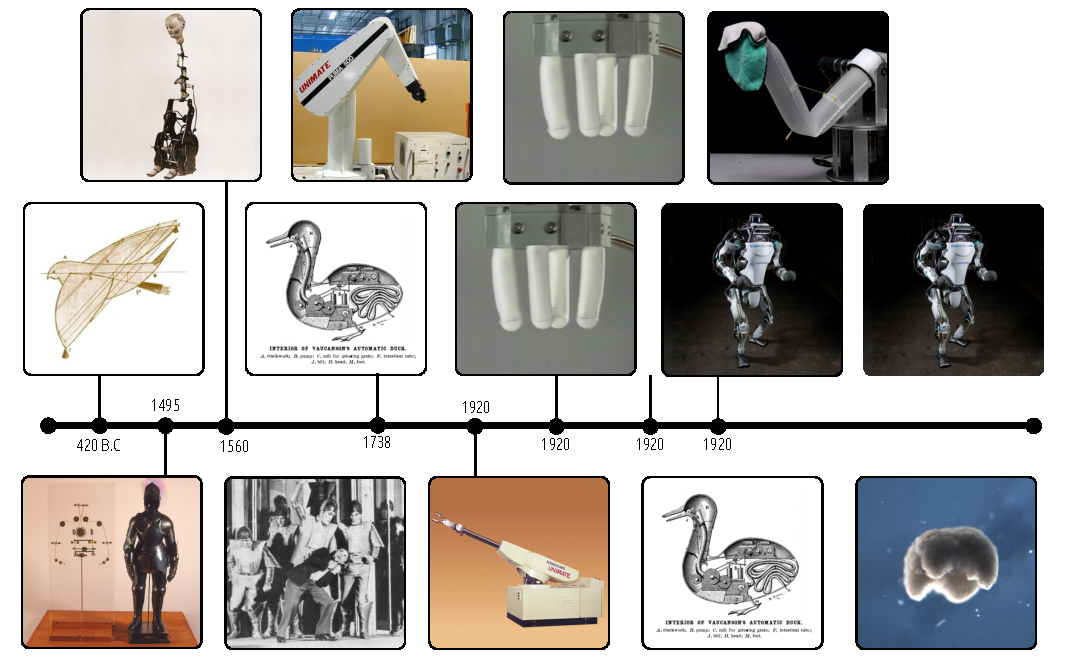
\includegraphics[width=1.0\textwidth]{./3_chapters/0_introduction/img/timeline.pdf}
\end{figure}
\clearpage
}

\subsection{REF}

\begin{itemize}
  \item . F. Shulte, "The Characteristics of the Mckibben Artificial Muscle", The Application of External Power in Prosthetics and Orthetics, pp. 94-115, 1960.
  \item A. Chen, R. Yin, L. Cao, C. Yuan, H. K. Ding and W. J. Zhang, "Soft robotics: Definition and research issues," 2017 24th International Conference on Mechatronics and Machine Vision in Practice (M2VIP), 2017, pp. 366-370, doi: 10.1109/M2VIP.2017.8267170.
\end{itemize}
